\documentclass[tikz,border=5]{standalone}
  \usepackage{xxcolor}
  \usetikzlibrary{arrows.meta}
  \tikzset{pics/cube/.style args={#1 #2 #3 #4}{code={%
    \path [#4, fill, draw]
      (0,#2,0)  coordinate (-top-a) -- (#1,#2,0) coordinate (-top-b) --
      (#1,#2,#3) coordinate (-top-c) -- (0,#2,#3) coordinate (-top-d) -- cycle;
    \path [#4!75!black, fill, draw]
      (#1,0,0) -- (#1,#2,0) -- (#1,#2,#3) -- (#1,0,#3) -- cycle;
    \path [#4!50!black, fill, draw]
      (0,0,#3) -- (0,#2,#3) -- (#1,#2,#3) -- (#1,0,#3) -- cycle;
  }}}
\begin{document}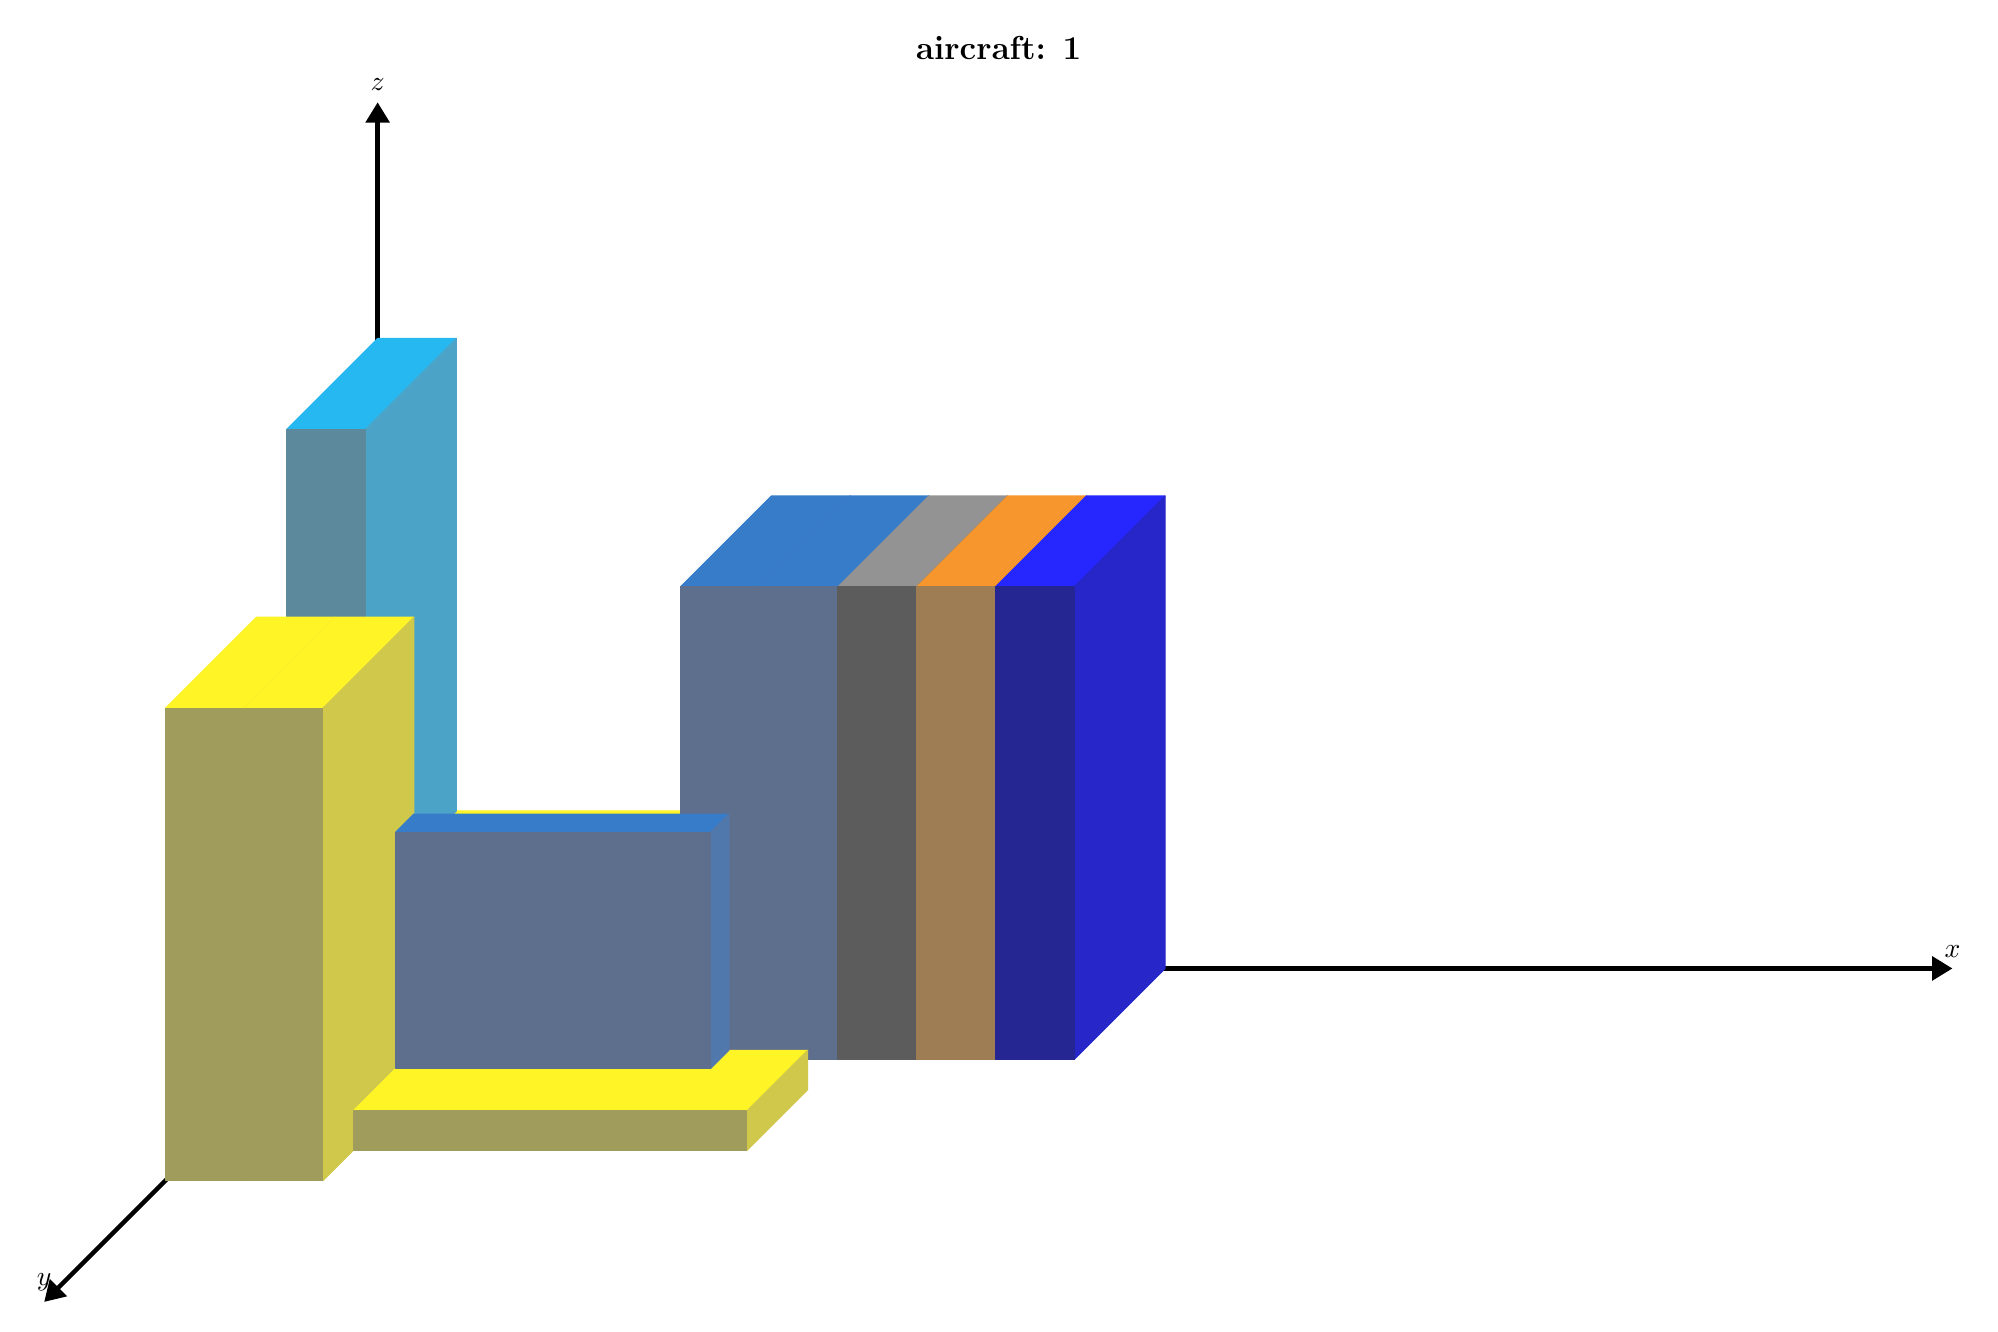
\begin{tikzpicture}[line join=round, line cap=round,>=Triangle,
   axis/.style={ultra thick, ->, draw=black}]
  \draw [axis] (0,0,0) -- (20.0,0,0) node (xaxis) [above] {$x$};
  \draw [axis] (0,0,0) -- (0,11.0,0) node (xaxis) [above] {$z$};
  \draw [axis] (0,0,0) -- (0,0,11.0) node (xaxis) [above] {$y$};
  \begin{colormixin}{85!white}\pic at (0,0,0) {cube={5.0 1.0 4.0 yellow!50!red}};
\pic at (0,1.0,0) {cube={5.0 1.0 4.0 yellow}};
\pic at (0,2.0,0) {cube={1.0 6.0 3.0 cyan}};
\pic at (5.0,0,0) {cube={1.0 6.0 3.0 cyan!50!blue}};
\pic at (6.0,0,0) {cube={1.0 6.0 3.0 cyan!50!blue}};
\pic at (7.0,0,0) {cube={1.0 6.0 3.0 gray}};
\pic at (8.0,0,0) {cube={1.0 6.0 3.0 yellow!50!red}};
\pic at (9.0,0,0) {cube={1.0 6.0 3.0 blue}};
\pic at (0,0,4.0) {cube={1.0 6.0 3.0 yellow}};
\pic at (1.0,0,4.0) {cube={1.0 6.0 3.0 yellow}};
\pic at (2.0,0,4.0) {cube={5.0 0.5 2.0 yellow}};
\pic at (2.0,0.5,4.0) {cube={4.0 3.0 0.5999999999999996 cyan!50!blue}};
\end{colormixin}
  \node[above,font=\large\bfseries] at (current bounding box.north) {aircraft: 1};
  \end{tikzpicture}\end{document}